\documentclass[tikz,border=2pt]{standalone}
\usepackage{amsmath}
\usepackage{pgfplots}
\pgfplotsset{compat=1.18}
\usetikzlibrary{arrows.meta}

\begin{document}
% Summary measures of the skewed density f(x) = x e^{-x}: centre (mode 1, median 1.68, mean 2),
% spread (standard deviation sqrt 2) and shape (right-skewed: mode < median < mean).
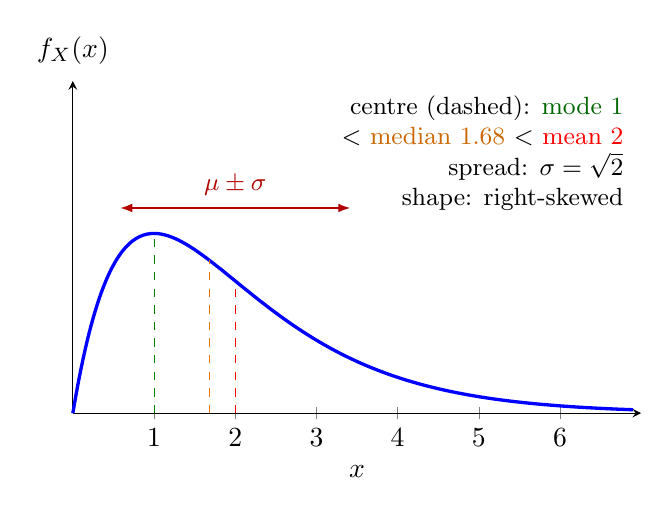
\begin{tikzpicture}
	\begin{axis}[
		axis lines=left, xmin=0, xmax=7, ymin=0, ymax=0.68,
		xtick={1,2,3,4,5,6}, ytick=\empty,
		xlabel={$x$}, ylabel={$f_X(x)$}, ylabel style={rotate=-90, anchor=south, at={(axis description cs:0,1.02)}},
		samples=160, smooth, width=8.8cm, height=5.8cm, clip=false
		]
		\addplot[blue, very thick, domain=0:6.9] {x*exp(-x)};
		\draw[green!50!black, dashed] (axis cs:1,0) -- (axis cs:1,0.368);
		\draw[orange!90!black, dashed] (axis cs:1.678,0) -- (axis cs:1.678,0.313);
		\draw[red, dashed] (axis cs:2,0) -- (axis cs:2,0.271);
		\draw[{Latex[length=1.5mm]}-{Latex[length=1.5mm]}, red!70!black] (axis cs:0.586,0.42) -- (axis cs:3.414,0.42);
		\node[red!70!black, font=\small, anchor=south] at (axis cs:2,0.425) {$\mu\pm\sigma$};
		\node[anchor=north east, font=\small, align=right] at (axis cs:6.9,0.67) {centre (dashed): \textcolor{green!40!black}{mode $1$}\\ $<$ \textcolor{orange!80!black}{median $1.68$} $<$ \textcolor{red}{mean $2$}\\ spread: $\sigma=\sqrt2$\\ shape: right-skewed};
	\end{axis}
\end{tikzpicture}
\end{document}
